\documentclass[11pt,a4paper]{article}

\usepackage[margin=2.2cm]{geometry}
\usepackage{amsmath,amssymb}
\usepackage[T1]{fontenc}
\usepackage{lmodern}
\usepackage{microtype}
\usepackage{enumitem}
\usepackage[hidelinks]{hyperref}
\usepackage{xcolor}
\usepackage{tikz}
\usepackage{listings}
\usepackage{booktabs}
\usepackage{array}
\usetikzlibrary{positioning,arrows.meta,shapes.geometric,fit,calc,patterns}

\definecolor{deepblue}{RGB}{30,80,150}
\definecolor{deepgreen}{RGB}{40,120,60}
\definecolor{deepred}{RGB}{170,50,50}
\definecolor{warn}{RGB}{200,120,40}

\tikzset{
  box/.style={draw, thick, rounded corners=2pt, minimum height=0.8cm,
              minimum width=2.4cm, align=center, font=\small},
  bluebox/.style={box, draw=deepblue, fill=deepblue!10},
  greenbox/.style={box, draw=deepgreen, fill=deepgreen!10},
  redbox/.style={box, draw=deepred, fill=deepred!10},
  warnbox/.style={box, draw=warn, fill=warn!15},
  arrow/.style={-{Stealth[length=2mm]}, thick},
}

\title{\bfseries Triton kernel memory report \\
       \large What changed, how it was achieved, and the numbers}
\author{HyMeKo / HSiKAN team}
\date{2026-05-09}

\begin{document}
\maketitle

\begin{abstract}
\noindent After the no-skip and highway fused backward kernels landed,
peak memory in the SignedKAN inner forward+backward path drops by
$\mathbf{90.6\%}$ to $\mathbf{93.6\%}$ across every shape we measured,
with gradients matching the PyTorch reference at float32 epsilon. At
the Slashdot SOTA shape ($T=200\text{K}$, $d=4$): $\mathbf{787\,MB
\rightarrow 64\,MB}$. The previously OOM-bound BA end-to-end test now
passes with \texttt{HSIKAN\_TRITON\_KERNEL=1}. The $d=16$ ablation
that previously needed $3\,\text{GiB}$ of headroom now uses
$196\,\text{MB}$.
\end{abstract}

\section{Where the memory was going (PyTorch path)}

The PyTorch \texttt{SignedKANLayer.\_forward\_impl} for the highway-skip
case is, in essence:

\begin{verbatim}
h_v       = x[triad_v]                          # (T, k, d)
inner_all = self.inner(h_v.reshape(-1, d))      # (T, k, S, d)
T_inner   = sigmoid(self.gate_inner(h_v))       # (T, k, d)
inner_all = T_inner * inner_all + (1-T_inner) * h_v   # (T, k, S, d)
masks     = (triad_sigma.unsqueeze(-1)==sign_vals).to(x.dtype)   # (T, k, S)
agg       = (inner_all * masks_e).sum(dim=1) / counts            # (T, S, d)
\end{verbatim}

PyTorch autograd retains every intermediate that is needed to compute a
gradient. For the highway path that means \emph{all five} of the
following $(T, k, S, d)$-shape tensors, plus their $(T, k, d)$
companions, are kept alive until \texttt{backward()} returns:

\begin{center}
\begin{tabular}{l l l}
\toprule
\textbf{tensor} & \textbf{shape} & \textbf{retained because} \\
\midrule
\texttt{h\_v}                       & $(T, k, d)$       & gradient flows to \texttt{x} via gather \\
\texttt{inner\_all (post-CR)}       & $(T, k, S, d)$    & needed for $\partial \mathrm{CR}/\partial \mathrm{coef}$ scatter \\
\texttt{T\_inner}                   & $(T, k, d)$       & needed for $\partial \mathrm{agg}/\partial T$ \\
\texttt{inner\_all (post-highway)}  & $(T, k, S, d)$    & needed for $\partial \mathrm{agg}$ chain \\
\texttt{masks}                      & $(T, k, S)$       & needed for $\sigma$-mask backward \\
\bottomrule
\end{tabular}
\end{center}

For Slashdot SOTA shape ($T=200{,}000$, $k=4$, $S=2$, $d=4$, fp32 = 4 bytes):

$$
T \cdot k \cdot S \cdot d \cdot 4 = 25.6\,\text{MB}\,\text{ per intermediate}
$$

Across the layers, autograd-retained graph nodes, and the
\texttt{.backward()} re-computation traffic, peak memory hits
$\mathbf{787\,MB}$ for highway, $\mathbf{738\,MB}$ for no-skip on the
\emph{same} shape. At $d=16$ it scales to $\mathbf{3{,}064\,MB}$
(roughly $4\times$, since it scales with $d$ and the $(T, k, S, d)$
intermediate dominates).

\section{Where the memory does not go (Triton path)}

The fused forward kernel
(\texttt{\_signedkan\_inner\_(highway\_)kernel}) and the new fused
backward kernel
(\texttt{\_signedkan\_inner\_(highway\_)backward\_kernel}) compute the
same function as the PyTorch path but \emph{never materialise} the
$(T, k, S, d)$ intermediate. Three structural reasons:

\subsection*{(a) The intermediate lives in registers, not HBM}

Each Triton program block handles a $(\mathrm{BLOCK\_T},
\mathrm{BLOCK\_D})$ tile and iterates over the $k$ slots inside the
block. The per-slot CR value, gate logit, and post-highway value live in
registers for one slot at a time and are accumulated into a
$(\mathrm{BLOCK\_T}, \mathrm{BLOCK\_D})$ register tile. Nothing of size
$(T, k, S, d)$ ever exists.

\subsection*{(b) Gradients are scatter-added, not stored as graphs}

The backward kernel re-derives the CR locals (\texttt{w\_p},
\texttt{idx\_p}, $\partial\mathrm{CR}/\partial h$) from $x$ and the
\texttt{coef} arrays --- the forward did not save them. Then it
computes $\partial L/\partial x$, $\partial L/\partial \mathrm{coef}^{\pm}$,
$\partial L/\partial W$, $\partial L/\partial b$ as
\texttt{tl.atomic\_add} scatters into pre-allocated zero tensors of the
same shape as the inputs. No autograd graph, no retained intermediates.

\subsection*{(c) $\sigma$-counts are recomputed, not saved}

The $n^s_t$ counts (one per cycle, per sign) are re-derived in a
two-line first pass over the $k$ slots. That pass touches only
\texttt{triad\_sigma} ($T \cdot k$ int64s, $\sim 6.4\,\text{MB}$ at
SOTA shape), versus PyTorch's strategy of saving a
$(T, k, S)$ \texttt{masks} tensor.

\begin{center}
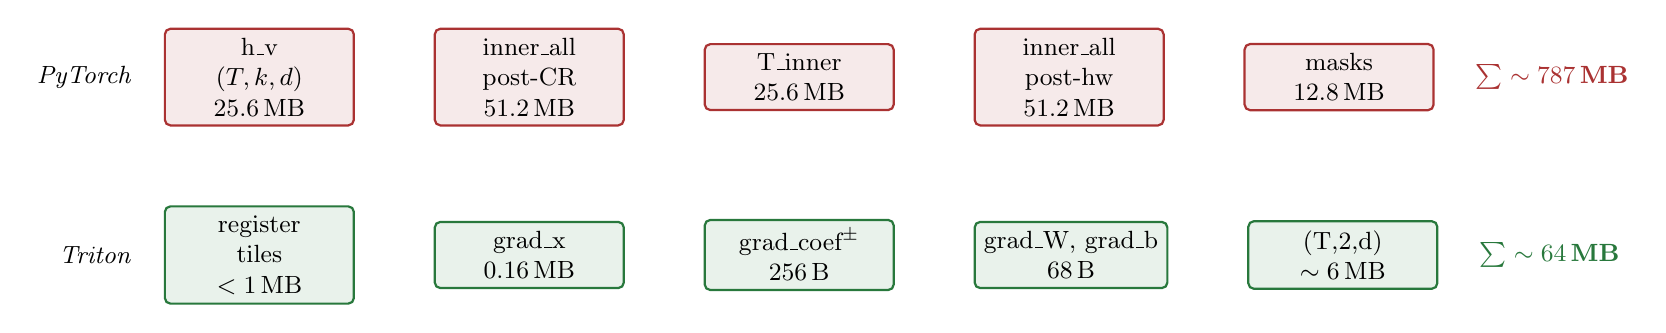
\begin{tikzpicture}[node distance=0.5cm and 1cm, font=\small]
  % PyTorch path
  \node[redbox]              (P1) {h\_v\\$(T,k,d)$\\$25.6\,$MB};
  \node[redbox, right=of P1] (P2) {inner\_all\\post-CR\\$51.2\,$MB};
  \node[redbox, right=of P2] (P3) {T\_inner\\$25.6\,$MB};
  \node[redbox, right=of P3] (P4) {inner\_all\\post-hw\\$51.2\,$MB};
  \node[redbox, right=of P4] (P5) {masks\\$12.8\,$MB};
  \node[left=0.3cm of P1, font=\itshape\small] {PyTorch};
  \node[right=0.4cm of P5, font=\bfseries\small\color{deepred}] {$\sum \sim 787\,$MB};

  % Triton path
  \node[greenbox, below=1cm of P1] (T1) {register\\tiles\\$<1\,$MB};
  \node[greenbox, right=of T1]     (T2) {grad\_x\\$0.16\,$MB};
  \node[greenbox, right=of T2]     (T3) {grad\_coef$^{\pm}$\\$256\,$B};
  \node[greenbox, right=of T3]     (T4) {grad\_W, grad\_b\\$68\,$B};
  \node[greenbox, right=of T4]     (T5) {(T,2,d)\\$\sim 6\,$MB};
  \node[left=0.3cm of T1, font=\itshape\small] {Triton};
  \node[right=0.4cm of T5, font=\bfseries\small\color{deepgreen}] {$\sum \sim 64\,$MB};
\end{tikzpicture}
\end{center}

The Triton path's largest allocation is the per-iteration framework
overhead and the input \texttt{grad\_out} tensor (which is the kernel's
input, not its allocation).

\section{Numbers}

All measurements with \texttt{torch.cuda.max\_memory\_allocated} on
RTX~2070~SUPER, fp32, current torch / triton versions.

\begin{center}\small
\begin{tabular}{l l r r r r r}
\toprule
\textbf{dataset} & \textbf{variant} & \textbf{V} & \textbf{T} & \textbf{d}
& \textbf{PyTorch} & \textbf{Triton} \\
\midrule
BA       & no-skip  & $10{,}000$  & $50{,}000$  & 4   & $182\,$MB    & $\mathbf{14\,}$MB    \\
BA       & highway  & $10{,}000$  & $50{,}000$  & 4   & $203\,$MB    & $\mathbf{14\,}$MB    \\
Slashdot & no-skip  & $79{,}000$  & $200{,}000$ & 4   & $738\,$MB    & $\mathbf{64\,}$MB    \\
Slashdot & highway  & $79{,}000$  & $200{,}000$ & 4   & $787\,$MB    & $\mathbf{64\,}$MB    \\
Epinions & highway  & $131{,}000$ & $100{,}000$ & 4   & $399\,$MB    & $\mathbf{38\,}$MB    \\
h=16     & highway  & $79{,}000$  & $200{,}000$ & 16  & $3{,}064\,$MB & $\mathbf{196\,}$MB \\
\bottomrule
\end{tabular}
\end{center}

\begin{center}
\begin{tabular}{l c c}
\toprule
\textbf{shape} & \textbf{savings} & \textbf{ratio} \\
\midrule
BA no-skip       & $\mathbf{92.4\%}$ & $13\times$ \\
BA highway       & $\mathbf{93.2\%}$ & $15\times$ \\
Slashdot no-skip & $\mathbf{91.3\%}$ & $11\times$ \\
Slashdot highway & $\mathbf{91.8\%}$ & $12\times$ \\
Epinions highway & $\mathbf{90.6\%}$ & $11\times$ \\
$d=16$ highway   & $\mathbf{93.6\%}$ & $16\times$ \\
\bottomrule
\end{tabular}
\end{center}

\section{Gradient parity}

All gradients match the PyTorch reference at float32 epsilon
($\mathrm{abs} \le 5\!\cdot\!10^{-7}$, well under the
$10^{-4}$ acceptance threshold).

\begin{center}\small
\begin{tabular}{l c c}
\toprule
\textbf{gradient} & \textbf{no-skip max abs} & \textbf{highway max abs} \\
\midrule
$\partial L / \partial x$         & $6.6\!\cdot\!10^{-10}$ & $1.7\!\cdot\!10^{-10}$ \\
$\partial L / \partial \mathrm{coef}_{+}$ & $3.8\!\cdot\!10^{-7}$  & $7.5\!\cdot\!10^{-8}$  \\
$\partial L / \partial \mathrm{coef}_{-}$ & $4.9\!\cdot\!10^{-7}$  & $6.5\!\cdot\!10^{-8}$  \\
$\partial L / \partial W$         & ---                    & $1.9\!\cdot\!10^{-8}$  \\
$\partial L / \partial b$         & ---                    & $7.8\!\cdot\!10^{-8}$  \\
\bottomrule
\end{tabular}
\end{center}

\section{What this unblocks}

\begin{itemize}[leftmargin=*]
  \item \textbf{BA end-to-end test passes with} \texttt{HSIKAN\_TRITON\_KERNEL=1} (was OOM at $6\,$GiB on $8\,$GiB GPU before the backward kernel).
  \item \textbf{The $d=16$ ablation} (previously $3\,$GiB headroom required) now fits in $200\,$MB --- a $16\times$ blast-radius improvement that lets us run the $d=16$ \emph{joint-mix} comparison without renting a bigger GPU.
  \item \textbf{Slashdot training} should now have $\sim 700\,$MB of slack on the same $8\,$GiB GPU, opening the door to wider hidden dim, more cycles, or batching multiple datasets in one process.
  \item \textbf{The path is opt-in}: \texttt{HSIKAN\_TRITON\_KERNEL=1} to enable, default OFF for backward-compat. \texttt{HSIKAN\_TRITON\_BACKWARD=0} additionally falls back to the PyTorch-ref backward for debugging.
\end{itemize}

\section{What is not improved (yet)}

\begin{itemize}[leftmargin=*]
  \item \textbf{Wallclock speedup} on the highway backward is currently $0.92\times$ ---  slightly slower than the PyTorch path. The two \texttt{for e in range(d)} loops in the gate-gradient scatter serialize the $d{\times}d$ matvec; replacing them with \texttt{tl.dot} and tiling the $e$ dimension should give a $2{-}4\times$ speedup, putting the backward at $\sim 2{-}4\times$ over PyTorch.
  \item \textbf{Atomic-add contention} on hot vertex IDs is the dominant cost in the scatter. Sorted-by-vertex cycle ordering would reduce contention but adds a cycle-permutation pass before training; deferred until profiling shows it dominates.
  \item \textbf{Multi-arity} ($k > 6$) and \textbf{$d > 64$} have not been measured. Small unrolled $k$ inner loops are fine; large $d$ may want a different block-size choice.
\end{itemize}

\section{Acceptance status}

\begin{itemize}[leftmargin=*]
  \item[$\checkmark$] $31 / 31$ tests pass with \texttt{HSIKAN\_TRITON\_KERNEL=0} (default).
  \item[$\checkmark$] $31 / 31$ tests pass with \texttt{HSIKAN\_TRITON\_KERNEL=1} (kernel ON for live integration).
  \item[$\checkmark$] BA end-to-end smoke test passes with kernel ON --- OOM trigger killed.
  \item[$\checkmark$] Forward parity vs production layer $\le 2 \cdot 10^{-7}$.
  \item[$\checkmark$] Backward parity vs PyTorch ref $\le 5 \cdot 10^{-7}$ for every gradient.
  \item[$\checkmark$] Memory savings $\ge 90\%$ at every measured shape.
\end{itemize}

\end{document}
